\nsecbegin{Was wird wie gemacht?}
\nsecbegin{Eclipse}
\nsecbegin{Projekt in Eclipse importieren}
In den workspace wecheln:\\
cd ~/workspace\\
Projekt Klonen:\\
git clone https://gitlab.imn.htwk-leipzig.de/weicker/puml.git\\
Benutzername und Passwort eingeben.\\
In Eclipse "File->Import->Existing Projects into Workspace"\\
%\begin{figure}[hbtp]
%\centering
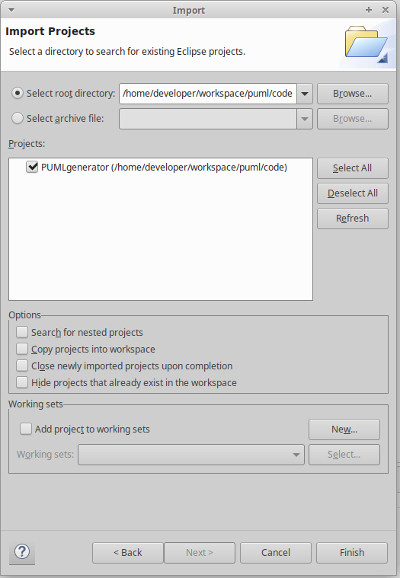
\includegraphics[scale=0.25]{Bilder/importProject}\\
%\caption{Projekt in Eclipse importieren}
%\end{figure}
Dann auf "'Finish"' klicken.
\nsecend

\nsecbegin{WindowBuilder installieren}
In Eclipse "Help->Install New Software..."\\
Unter work with "'2018-09 - http://download.eclipse.org/releases/2018-09"' auswählen.\\
In der Section "'General Purpose Tools"' die im Bild stehenden Häckchen anklicken\\	
\begin{figure}[hbtp]
\centering
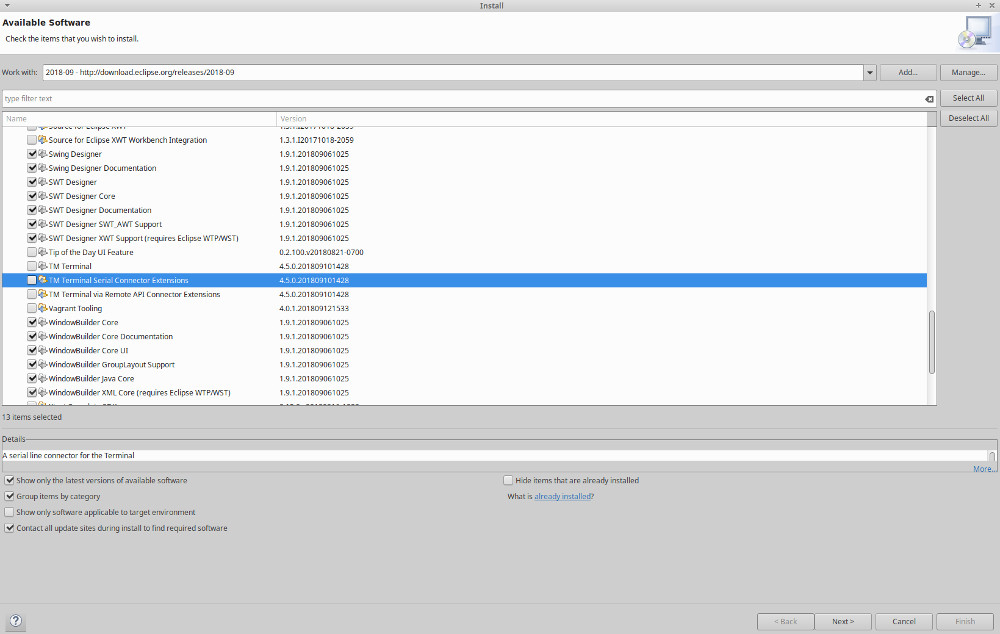
\includegraphics[scale=0.4]{Bilder/installWindowBuilder}\\
\caption{WindowBuilder installieren}
\end{figure}
Dann auf "'Finish"' und sich durch die Installation klicken.
\nsecend

\nsecbegin{GUI editieren}
Es muss der WindowBuilder installiert sein. Dann auf die Datei die die Grafische Oberfläche implementiert (GUI.java) mit der rechten Maustaste klicken. Dann "'Open With->WindowBuilder Editor"' auswählen.
\nsecend
\nsecend

\nsecend